\chapter{Development and code with lstlistings}\label{dev}

I'l write after a comment in that language and a \lstinline{@} the location the code is either written or executed in.

Some Japanese text: 日本語の文書 is displayed normally in XeLaTeX

\begin{lstlisting}[language=bash, title={small Execute in: bash}]
# @ ~/some-directory

echo 'Hello World!' # ここも also in listings, if using XeLaTeX
\end{lstlisting}

Parenthesis for the branch if it's using git \lstinline{git}:

\begin{lstlisting}[language=bash, title={small Execute in: bash}]
# @ ~/some-directory (branch)

echo 'Hello World!'
\end{lstlisting}

If\lstinline{venv} has \lstinline{activate} :

\begin{lstlisting}[language=bash, title={small Execute in: bash}]
# @ ~/some-directory (venv)

echo 'Hello World!'
\end{lstlisting}

If inside a file:
\begin{lstlisting}[language=python, title={small Language: python}]
# @ ~/some-directory/some_file.py

print('Hello World!')
\end{lstlisting}

If inside a method or class inside a file:

\begin{lstlisting}[language=python, title={small Language: python}]
# @ ~/some-directory/some_file.py :: class HelloWorld:

def display():
    print('Hello World!')
\end{lstlisting}

\begin{lstlisting}[language=python, title={small Language: python}]
# @ ~/some-directory/some_file.py :: class HelloWorld: display():

print('Hello World!')
\end{lstlisting}

If location isn't relevant:

\begin{lstlisting}[language=bash, title={small Execute in: bash}]
echo 'Hello World!'
\end{lstlisting}


\section{Project layout}\label{dev-layout}

CMD: \lstinline{tree /F /A | clip} 

\begin{lstlisting}[]
~/my-project
|   .gitignore
|   MANIFEST.in
|   README.md
|   requirements.txt
|   setup.cfg
|   setup.py
|   
+---logs
|       tasklog.md
|       ...
|   
+---manual_tests
|   |   ...
|   |   ProjectPaths.py
|   |   UsefulMethods.py
|   \---__pycache__
|           ...
|   
+---report
|   |   report.tex
|   |   report.bib
|   \---...
|       
+---package-name
|   |   action.py
|   |   __init__.py
|   |   
|   +---static
|   |       css_test.html
|   |       style.css
|   |       
|   +---templates
|   |       layout.html
|   |       action.html
|   |       
|   \---__pycache__
|           ...
|       
+---tests
|   |   conftest.py
|   |   test_factory.py
|   \---__pycache__
|           ...
|           
\---venv
       ...
\end{lstlisting}

\section{Design and multiple subfigures in one}\label{dev-css}

\subsection{HTML and CSScode with nice colors:}

\begin{lstlisting}[language=HTML5, title={small Language: HTML}]
<!-- @ ~/my-project/package-name/templates/search.html -->

<form id="search_bar" method="post">
    <div class="col-label">
        <label for="search_bar_q">Search term:</label>
    </div>
    <div class="col-input">
        <input type="text" id="search_bar_q" name="q" value="{{ request.form['q'] }}" placeholder="Search...">
    </div>
    <div class="col-submit">
        <button type="submit">Submit</button>
    </div>
</form>
\end{lstlisting}

\begin{lstlisting}[language=CSS, title={small Language: CSS}]
/* @ ~/my-project/package-name/static/style.css */

form {
    width: 100%;
}

.col-label {
    display: inline-block;
    width: 20em;
}

.col-input {
    display: inline-block;
    width: 50%;
}

.col-submit{
    display: inline-block;
    width: 10%;
}
\end{lstlisting}

\subsection{Design color: multiple figures}

\href{https://paletton.com}{Palletton} \cite[][]{paletton}.

Color Scheme in fig. \ref{fig:color-scheme} Simulations for color blindness in fig. \ref{fig:color-scheme-simulations}.

\begin{figure}[bh]
\centering
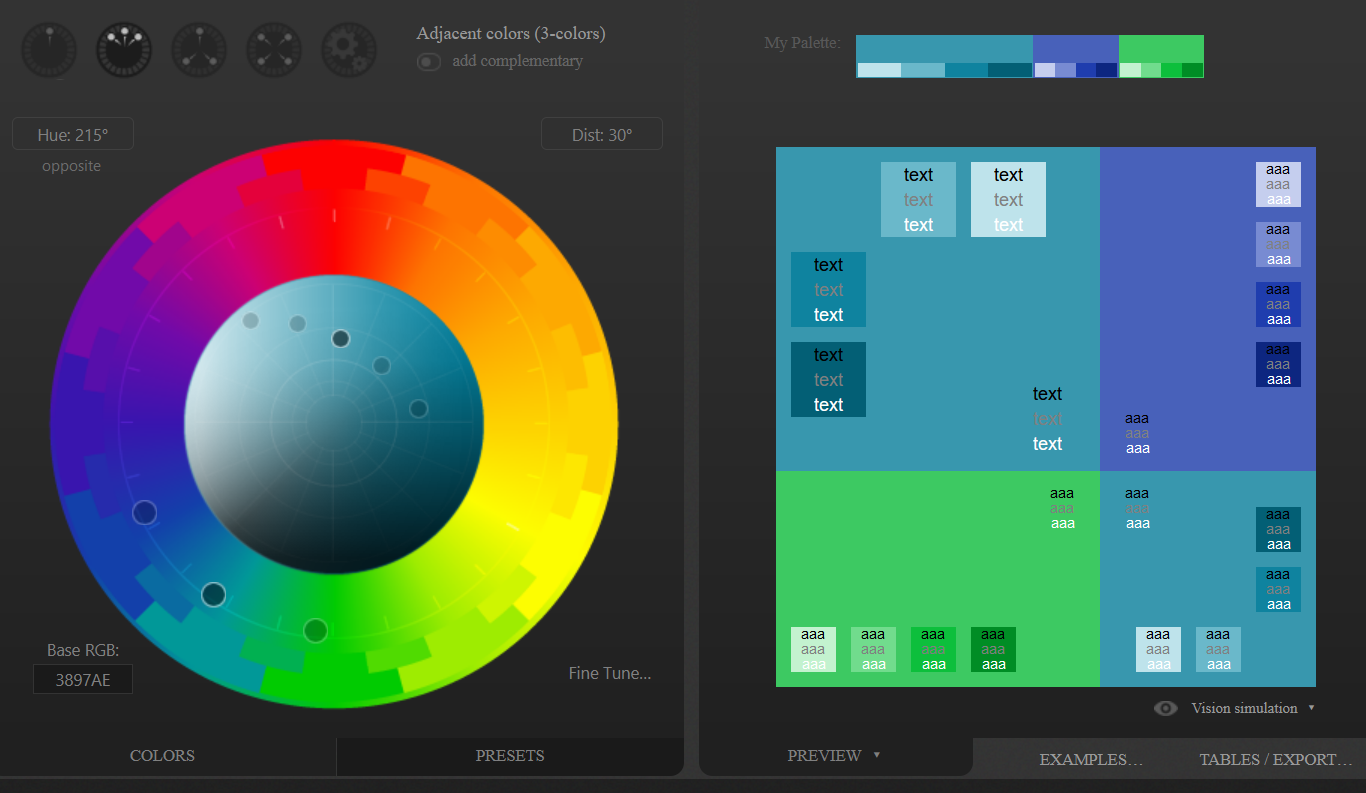
\includegraphics[width=0.8\linewidth]{figures/color-scheme.png}
\caption{Color scheme}
\label{fig:color-scheme}
\end{figure}

\begin{figure}[bh]
    \centering
    \begin{subfigure}[b]{0.4\linewidth}
        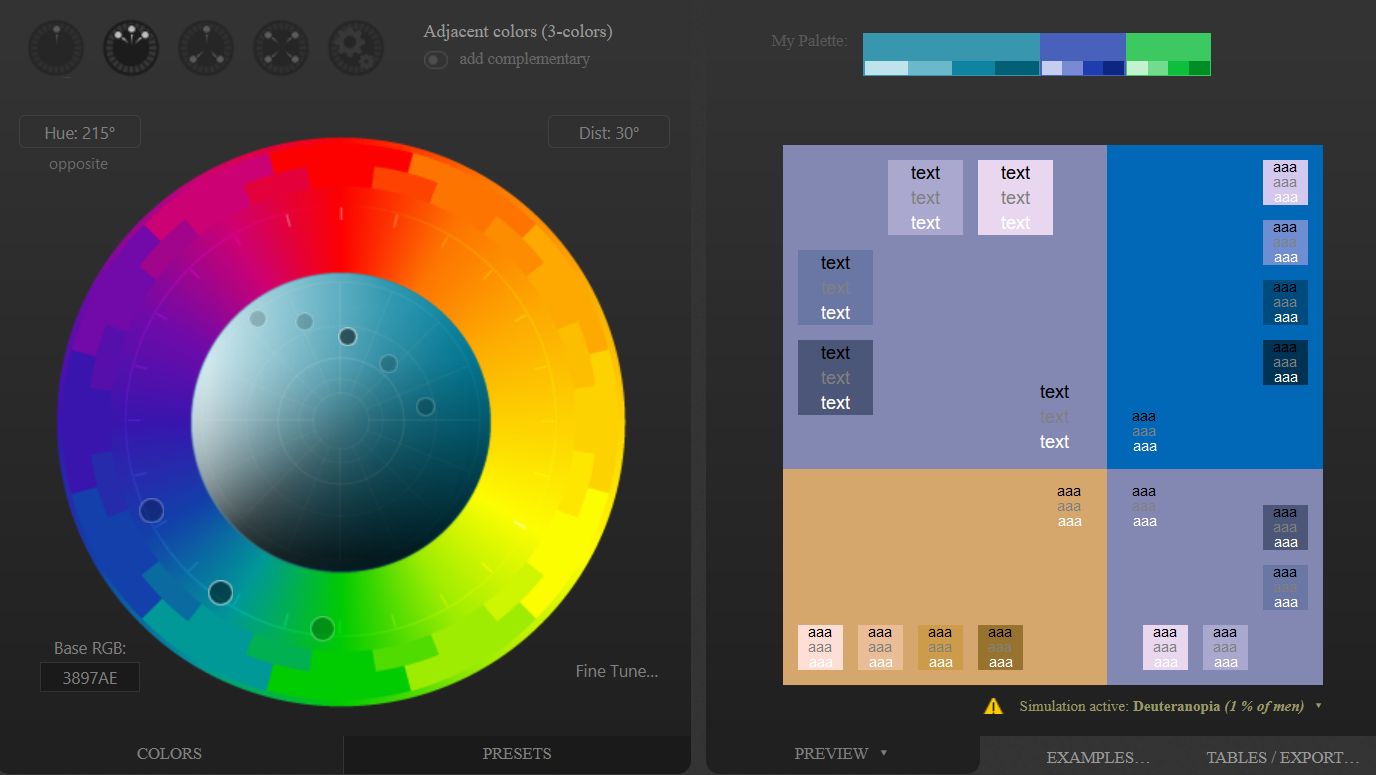
\includegraphics[width=\linewidth]{figures/color-scheme-deuteranopia.png}
        \caption{Deuteranopia}
    \end{subfigure}
    \begin{subfigure}[b]{0.4\linewidth}
        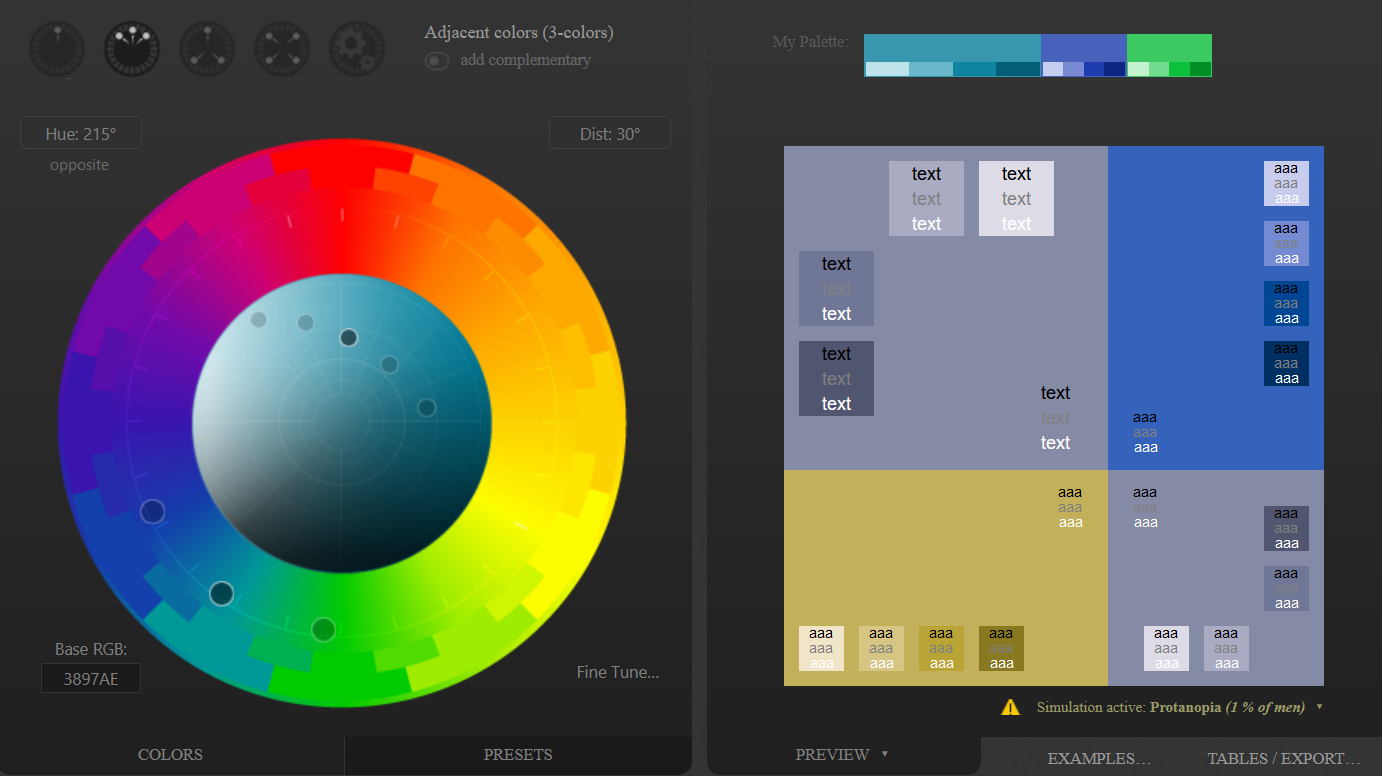
\includegraphics[width=\linewidth]{figures/color-scheme-protanopia.png}
        \caption{Protanopia}
    \end{subfigure}
    \begin{subfigure}[b]{0.4\linewidth}
        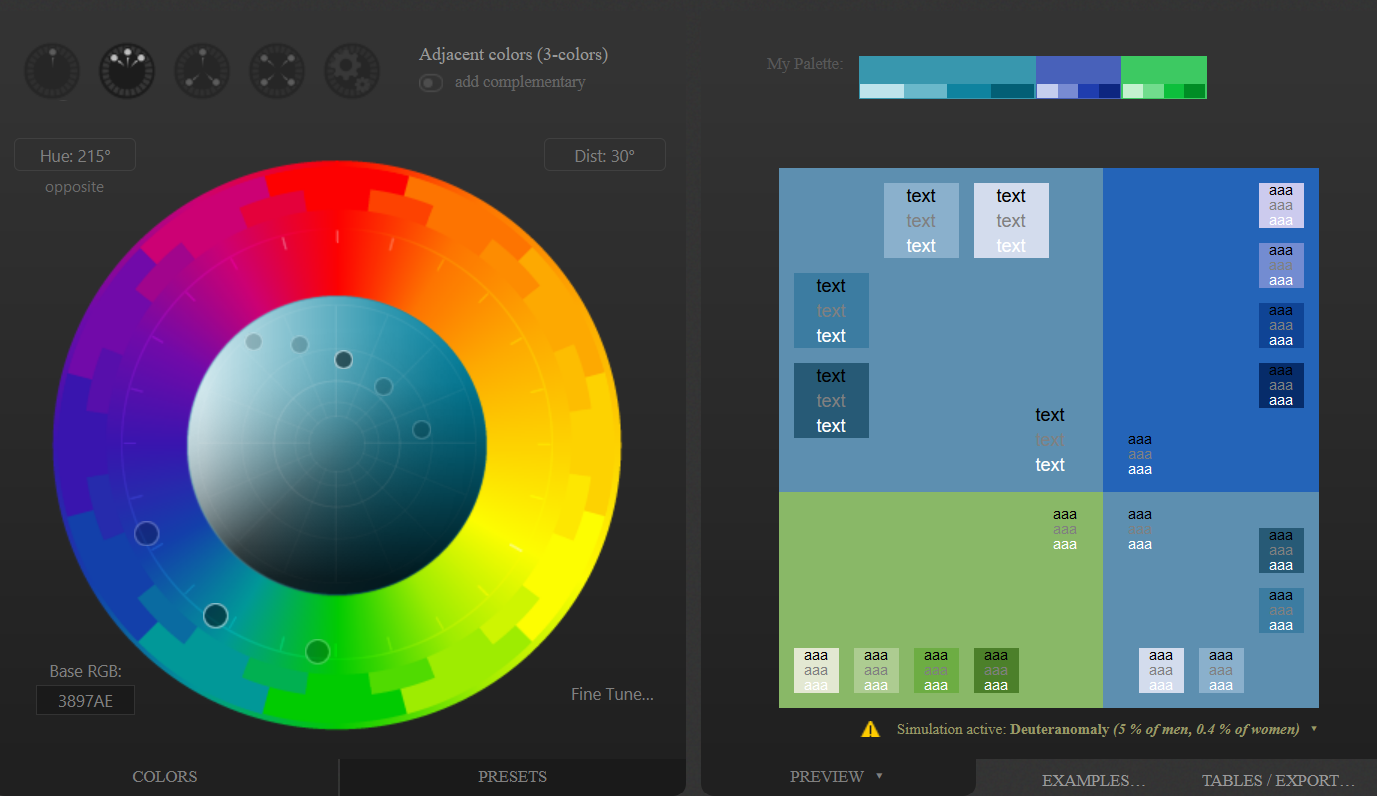
\includegraphics[width=\linewidth]{figures/color-scheme-deuteranomaly.png}
        \caption{Deuteranomaly}
    \end{subfigure}
    \begin{subfigure}[b]{0.4\linewidth}
        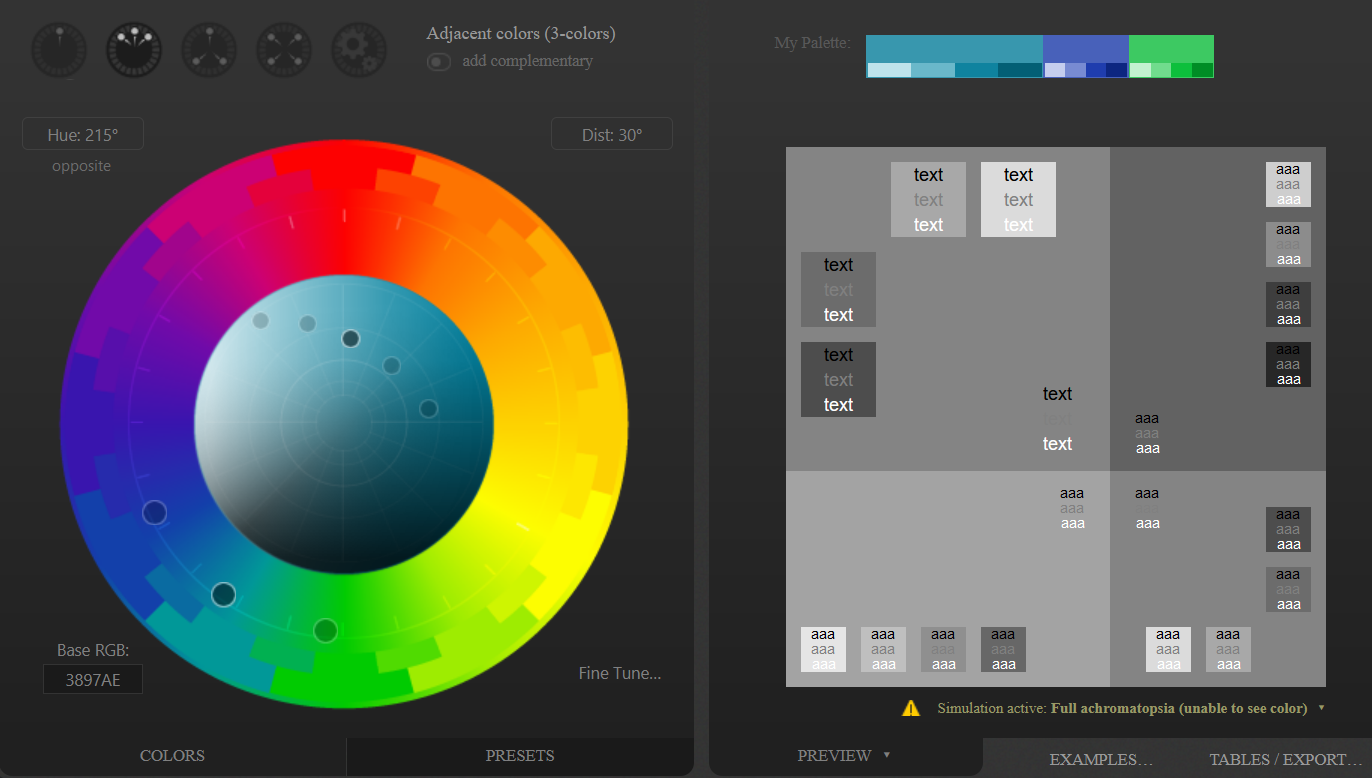
\includegraphics[width=\linewidth]{figures/color-scheme-achromatopsia.png}
        \caption{Achromatopsia}
    \end{subfigure}
\caption{Color Blindness Simulations}
\label{fig:color-scheme-simulations}
\end{figure}

%%%%%%%%%%%%%%%%%%%%%%%%%
%%%%%%%%%%%%%%%%%%%%%%%%%
%%%%%%%%%%%%%%%%%%%%%%%%%